\documentclass{article}
\usepackage[utf8]{inputenc}
\usepackage[spanish,CO]{babel}
\usepackage{listings}
\usepackage{graphicx}
\graphicspath{ {images/} }
\usepackage{cite}

\begin{document}

\begin{titlepage}
    \begin{center}
        \vspace*{1cm}
        
        \Huge
        \textbf{Arduino}
        
        \vspace{0.5cm}
        \LARGE
        Consulta
            
        \vspace{1.5cm}
            
        \textbf{Santiago Tangarife Guerra}
            
        \vfill
            
        \vspace{0.8cm}
            
        \Large
        Departamento de Ingeniería Electrónica y Telecomunicaciones\\
        Universidad de Antioquia\\
        Medellín\\
        Septiembre de 2020
            
    \end{center}
\end{titlepage}

\tableofcontents

\section{Sección introductoria}
Arduino es Hardware micro controlador de pulsos Eléctricos de muchas funciones en la electrónica y la robótica, personalmente desconozco casi todas sus funciones, y en este trabajo expondré una de ellas; que es imprimir texto en una pantalla LCD. Para este trabajo modifique un ejemplo de un trabajo ya creado.\cite{webpage}

\section{Sección de contenido} \label{contenido}

\vspace{0,5cm}
        \begin{align}

        \LARGE
        Para su construcción física:
        
        \end{align}
\vspace{0,2cm}

Para su construcción es necesario tener los componentes adecuados que listare a continuación y además saberlos instalar también es fundamental para que funcione correctamente.\\
\\ Los componentes necesarios son: \\
-Arduino uno R3\\
-Protoboard\\
-LCD 16x2\\
-Potenciómetro\\
-Resistencia 220 ohm\\
-Cables de conexión\\

\vspace{0,5cm}
        \begin{align}

        \LARGE
        Consideraciones en el desarrollo del software:
        
        \end{align}
\vspace{0,2cm}

Para el desarrollo del código se necesitan conocimientos básicos del lenguaje c++ y el lenguaje del microcontrolador.\\
A continuación, mostrare y explicare las partes del código:

\vspace{2cm}

\begin{lstlisting}
// llama la libreria liquidcrystal.
#include <LiquidCrystal.h>

// Inicializa la libreria con los numeros de los pines de la interfaz.
LiquidCrystal lcd(12, 11, 5, 4, 3, 2);

void setup() 
{
  // configura el numero de columnas y filas de la LCD:
  lcd.begin(16, 2);
  // Muestra el mensaje en la LCD.
  lcd.print("Santiago");
}

void loop() {}
\end{lstlisting}


\section{Conclusión} \label{conclulsion}
Una de las múltiples funciones de c++ en combinación con Arduino es mostrar texto en una pantalla LCD.\\
Por último, muestro una imagen del resultado del proceso.

\begin{figure}[h]
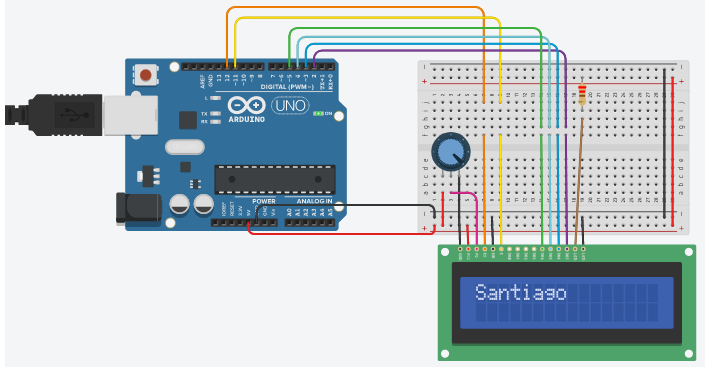
\includegraphics[width=12cm]{Captura.PNG}
\centering
\caption{Imagen del trabajo} \cite{webpage}
\label{fig:cpplogo}
\end{figure}
\bibliographystyle{IEEEtran}
\bibliography{references}
\end{document}